% L3a lecture companion deck.
% Follows the lecture: exchanges and securities; growth rates; risk;
% heavy tails, autocorrelation, and volatility clustering; examples and summary.
% Volatility conventions and the distribution comparison match the lecture.
% Title and disclaimer remain near the front by course convention.
% See lectures/templates/vnslides.sty for the shared content and style rules.
\documentclass[aspectratio=169,11pt]{beamer}
\usepackage{vnslides}

\title{{\vnheavy L3a}: Equity Exchanges, Growth Rates, and Stylized Facts}
\subtitle{CHEME 5660 Cornell University}
\author{Copyright Jeffrey Varner 2026. All Rights Reserved}

\begin{document}

% ==== title ==================================================
\vntitlepage

% ==== disclaimer =============================================
\begin{frame}{Disclaimer and Risks}
  \vspace{0.6em}
  \textbf{\ink{Training only.}} This content is for training and informational
  purposes only. The teaching team does not make, give, or endorse any offer or
  solicitation to buy or sell securities or derivative products, or provide
  investment or trading advice or strategy.

  \vspace{1.1em}
  \textbf{\ink{Risk.}} Trading involves risk and is generally not recommended for
  those with limited resources, experience, or a low risk tolerance. Past
  performance does not guarantee future success.

  \vspace{1.1em}
  \textbf{\ink{Responsibility.}} You are responsible for your investment decisions
  based on your financial circumstances, objectives, risk tolerance, and
  liquidity needs.
\end{frame}

% ==== objectives =============================================
\begin{frame}{Objectives for Today}
  Today we connect equity prices, growth rates, and the patterns a useful
  market model should reproduce.

  \vspace{0.9em}
  {\large\textbf{\ink{Today's concepts}}}
  \vspace{0.4em}
  \begin{itemize}\setlength{\itemsep}{0.7em}
    \item \hilite{Equity securities}: explain what stocks and ETFs represent
      and how they trade.
    \item \hilite{Growth rates and log returns}: compute both from prices
      and state their units.
    \item \hilite{Stylized facts}: identify heavy tails, weak growth-rate
      autocorrelation, and volatility clustering.
  \end{itemize}

  \slidenote{Lecture:}{\href{https://github.com/varnerlab/CHEME-5660-CourseRepository-Fall-2026/blob/main/lectures/week-3/L3a/CHEME-5660-L3a-Lecture-Equity-Exchanges-Return-StylizedFacts-Fall-2026.ipynb}{Equity Exchanges, Growth Rates, and Stylized Facts}}
\end{frame}

% ==== examples ===============================================
\begin{frame}{Lectures and Examples}
  \textbf{\ink{Lecture:}}
  \href{https://github.com/varnerlab/CHEME-5660-CourseRepository-Fall-2026/blob/main/lectures/week-3/L3a/CHEME-5660-L3a-Lecture-Equity-Exchanges-Return-StylizedFacts-Fall-2026.ipynb}{Equity Exchanges, Growth Rates, and Stylized Facts}

  \vspace{1.1em}
  \textbf{\ink{Example:}}
  \href{https://github.com/varnerlab/CHEME-5660-CourseRepository-Fall-2026/blob/main/lectures/week-3/L3a/CHEME-5660-L3a-SVD-SP500-Example-Fall-2026.ipynb}{SVD of S\&P 500 Growth Rates}

  Find common patterns across firms and reconstruct the growth-rate matrix
  using its leading modes.

  \vspace{1.1em}
  \textbf{\ink{Example:}}
  \href{https://github.com/varnerlab/CHEME-5660-CourseRepository-Fall-2026/blob/main/lectures/week-3/L3a/CHEME-5660-L3a-StylizedFacts-Example-Fall-2026.ipynb}{Stylized Facts in Daily Growth Rates}

  Compare distributions, estimate tail indices, and compare the ACF of
  growth rates with the ACF of their magnitudes.
\end{frame}

% ==== market structure =======================================
\begin{frame}{Exchanges, Stocks, and ETFs}
  \vspace{0.3em}
  Before measuring an equity return, separate the \hilite{marketplace} from the
  \hilite{securities} traded there.

  \vspace{0.7em}
  \begin{itemize}\setlength{\itemsep}{0.6em}
    \item An \hilite{exchange} is an organized venue that matches orders to buy
      and sell securities.
    \item An \hilite{order} is an investor's instruction to buy or sell a
      security. Order types differ in how they set the price.
    \item A \hilite{stock} is a residual ownership claim on a corporation.
    \item An \hilite{exchange-traded fund}, or ETF, is a security whose shares
      represent an interest in a portfolio and trade during the day.
  \end{itemize}

  \slidenote{Today:}{a market price is the price available at a particular time and trading venue.}
\end{frame}

\begin{frame}{\large Exchanges Connect Buyers and Sellers}
  Exchanges match buy and sell orders. Trading helps establish prices
  (\hilite{price discovery}) and lets investors trade with limited price impact
  (\hilite{liquidity}).

  \vspace{0.7em}
  \begin{itemize}\setlength{\itemsep}{0.7em}
    \item Exchanges set listing standards and trading rules.
    \item NYSE, Nasdaq, and Cboe each operate multiple venues.
      Cboe BZX is one venue within the Cboe group.
    \item Orders can be routed to different venues based on prices,
      available quantities, and order instructions.
  \end{itemize}

  \slidenote{Source:}{\href{https://www.sec.gov/about/divisions-offices/division-trading-markets/national-securities-exchanges}{SEC registered exchanges}. Clearing and settlement transfer the securities and funds after a trade.}
\end{frame}

\begin{frame}{Orders Are Instructions to Trade}
  An order states what to trade, whether to buy or sell, how much,
  and any price limits.

  \vspace{0.8em}
  \begin{itemize}\setlength{\itemsep}{0.8em}
    \item \textbf{\ink{Market order:}} seeks an immediate trade at available
      prices. A large order may trade at several prices.
    \item \textbf{\ink{Limit order:}} buys at the limit price or lower,
      or sells at the limit price or higher. It may not execute.
    \item \textbf{\ink{Stop and stop-limit orders:}} become market or limit
      orders when the price reaches a trigger.
  \end{itemize}

  \slidenote{Source:}{\href{https://www.investor.gov/introduction-investing/investing-basics/how-stock-markets-work/types-orders}{Investor.gov, Types of Orders}}
\end{frame}

\begin{frame}{Order Books and the NBBO}
  An \hilite{order book} holds outstanding buy and sell limit orders.
  Each venue keeps its own book.

  \vspace{0.7em}
  \begin{itemize}\setlength{\itemsep}{0.65em}
    \item \hilite{Bid}: the highest displayed buy price.
      \hilite{Ask}: the lowest displayed sell price.
      The spread is ask minus bid.
    \item A market buy begins at the best ask; a market sell begins at the
      best bid. Larger orders may use deeper price levels.
    \item The \hilite{National Best Bid and Offer (NBBO)} gives the highest
      displayed bid and lowest displayed ask across the national market system.
  \end{itemize}

  \slidenote{Order protection and best execution:}{\href{https://www.sec.gov/rules-regulations/2005/06/regulation-nms}{Regulation NMS} and \href{https://www.finra.org/rules-guidance/rulebooks/finra-rules/5310}{FINRA Rule 5310}. The NBBO is a quote benchmark.}
\end{frame}

\begin{frame}{Order Books and the NBBO for Stock XYZ}
  \vspace{0.1em}
  \begin{center}
    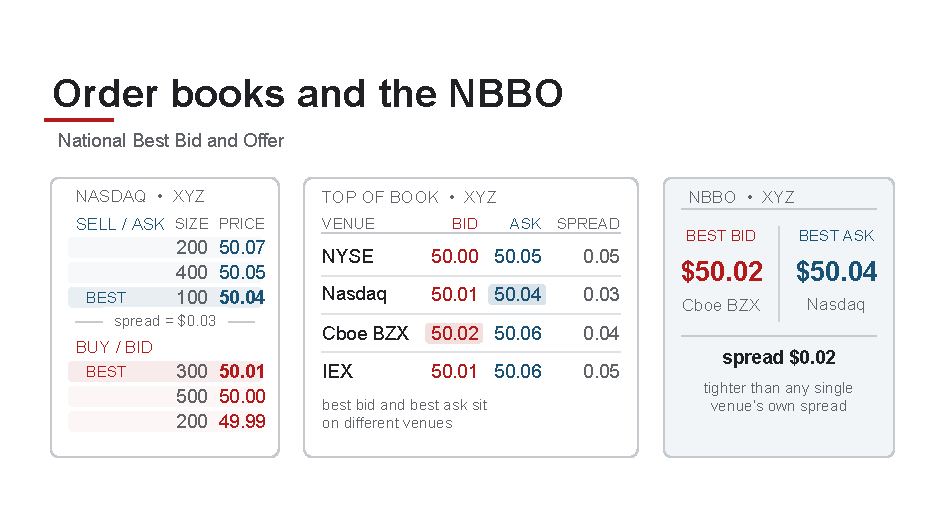
\includegraphics[width=0.84\textwidth,keepaspectratio]{../figs/Fig-L3a-Equity-Market-Schematic.pdf}
  \end{center}
\end{frame}

\begin{frame}{Stocks Are Claims on Firms}
  \vspace{0.4em}
  A stock, also called a share or \hilite{equity security}, represents fractional
  ownership in a corporation. It is a residual claim, not a promise of fixed
  repayment.

  \vspace{0.8em}
  {\large\textbf{\ink{What the shareholder may receive}}}
  \vspace{0.3em}
  \begin{itemize}\setlength{\itemsep}{0.5em}
    \item Voting rights and cash distributions such as dividends.
    \item A claim on remaining assets only after contractual creditors are paid.
    \item A capital gain if another investor later pays a higher share price.
  \end{itemize}

  \vspace{0.5em}
  Limited liability ordinarily caps the shareholder's loss at the invested
  amount. It does not protect the share price from falling to zero.

  \slidenote{Source:}{\href{https://www.investor.gov/introduction-investing/investing-basics/investment-products/stocks}{U.S. Securities and Exchange Commission, Stocks}}
\end{frame}

\begin{frame}{ETFs Are Claims on Portfolios}
  An ETF holds a portfolio and issues shares that trade throughout the day.

  \vspace{0.7em}
  \begin{itemize}\setlength{\itemsep}{0.7em}
    \item \hilite{Exposure}: broad-market funds such as SPY hold hundreds of
      stocks. Sector and single-stock ETFs are more concentrated.
    \item \hilite{Leveraged and inverse funds}: use derivatives to target
      a multiple or the negative of a stock's or index's daily move.
    \item \hilite{Net asset value (NAV)}: assets minus liabilities, divided
      by shares outstanding. The market price can be above or below NAV.
  \end{itemize}

  \vspace{0.6em}
  An ETF's risk depends on what it holds and how it invests.
\end{frame}

% ==== reward =================================================
\begin{frame}{Reward}
  \vspace{0.3em}
  We now turn from how shares trade to how their prices change. We measure
  that change with the \hilite{continuously compounded growth rate}, $g$.
  Let $S_{j-1}^{(i)}>0$ and $S_j^{(i)}>0$ be consecutive prices
  for firm $i$, $\Delta t_j>0$ years apart. The next price is given by:
  \[
    S_j^{(i)}=S_{j-1}^{(i)}\exp\!\left(g_{j,j-1}^{(i)}\Delta t_j\right).
  \]

  Solving for the growth rate gives the expression:
  \[
    g_{j,j-1}^{(i)}=
    \underbrace{\frac{1}{\Delta t_j}\log\!\left(\frac{S_j^{(i)}}{S_{j-1}^{(i)}}\right)}_{\text{\footnotesize growth rate}}.
  \]

  The growth rate has units of inverse years. Its sign records whether the price
  increased, decreased, or remained unchanged. The notebook computes $g$ from
  closing-price series, so dividends and other cash distributions are not
  included.
\end{frame}

\begin{frame}{Growth Rates and Log Returns}
  Let $g_t$ be the continuously compounded growth rate over an interval of
  length $\Delta t_t>0$ years. The corresponding \hilite{log return} $r_t$ is
  dimensionless and is given by:
  \[
    \underbrace{r_t=(\Delta t_t)g_t}_{\text{\footnotesize log return}}
    =\log\!\left(\frac{S_t}{S_{t-1}}\right).
  \]

  Log returns add across adjacent intervals. For positive prices
  $S_1,\ldots,S_T$, the cumulative log return is given by:
  \[
    \sum_{t=2}^{T}r_t
    =\underbrace{\sum_{t=2}^{T}(\Delta t_t)g_t}_{\text{\footnotesize time-weighted growth}}
    =\log\!\left(\frac{S_T}{S_1}\right).
  \]

  Use $g$ to compare annualized rates. Convert to $r$ before aggregating across
  time.
\end{frame}

\begin{frame}{Excess Growth Rate}
  To compare performance with a benchmark, subtract its growth rate.

  Let $g_t$ be the equity growth rate and $g_y$ the benchmark growth rate,
  both in inverse years. Over $\Delta t$ years, the excess growth rate
  and excess log return are given by:
  \[
    \underbrace{\bar g_t=g_t-g_y}_{\text{\footnotesize excess growth rate}},
    \qquad
    \underbrace{\bar r_t=(\Delta t)\bar g_t}_{\text{\footnotesize excess log return}}.
  \]

  \vspace{0.5em}
  \begin{itemize}\setlength{\itemsep}{0.6em}
    \item $\bar g_t>0$: the equity grew faster than the benchmark.
    \item $\bar g_t<0$: the equity grew more slowly.
    \item $\bar g_t=0$: their growth rates were equal.
  \end{itemize}

  \slidenote{Comparison:}{use the same currency, observation interval, and time units.}
\end{frame}

\begin{frame}{Algorithm}
  Given prices $\mathcal D_i=\{S_1^{(i)},\ldots,S_T^{(i)}\}$ for firm $i$,
  an interval $\Delta t>0$ years, and benchmark rate $g_y$ in inverse years:

  \vspace{0.6em}
  \begin{enumerate}\setlength{\itemsep}{0.6em}
    \item For each $t=2,\ldots,T$, read consecutive prices
      $S_{t-1}^{(i)}$ and $S_t^{(i)}$.
    \item Compute the excess growth rate using:
      \[
        \bar g_t^{(i)}\gets
        \underbrace{\frac{1}{\Delta t}\ln\!\left(\frac{S_t^{(i)}}{S_{t-1}^{(i)}}\right)}_{g_t^{(i)}}-g_y.
      \]
    \item Store the result. The $T$ prices give $T-1$ growth rates.
  \end{enumerate}

  Set $g_y=0$ to compute ordinary growth rates.
\end{frame}

\begin{frame}{Common Patterns Across Many Assets}
  Computing growth rates across firms lets us look for shared patterns.
  The matrix $\mathbf G\in\mathbb R^{m\times n}$ holds the observed growth rates
  for $m$ trading-day intervals and $n$ firms.

  In the singular value decomposition (SVD), columns $\mathbf u_j$ of
  $\mathbf U$ describe time patterns. Columns $\mathbf v_j$ of $\mathbf V$
  give firm weights. The diagonal entries $\sigma_j$ of $\boldsymbol\Sigma$
  give the size of each pattern. Together, these give the decomposition:
  \[
    \mathbf G=\mathbf U\boldsymbol\Sigma\mathbf V^{\mathsf T}
    =\sum_{j=1}^{\operatorname{rank}(\mathbf G)}
      \underbrace{\sigma_j\mathbf u_j\mathbf v_j^{\mathsf T}}_{\text{\footnotesize one mode}},
    \qquad \sigma_1\geq\sigma_2\geq\cdots\geq0.
  \]

  Keeping the leading modes gives a simpler approximation of the matrix.

  \slidenote{Example:}{\href{https://github.com/varnerlab/CHEME-5660-CourseRepository-Fall-2026/blob/main/lectures/week-3/L3a/CHEME-5660-L3a-SVD-SP500-Example-Fall-2026.ipynb}{SVD of S\&P 500 Growth Rates}. Shared patterns do not by themselves explain economic causes.}
\end{frame}

% ==== risk ===================================================
\begin{frame}{Risk}
  Shared patterns describe how firms move together. For each firm,
  volatility measures how widely growth rates vary around their mean.

  Let $g_2,\ldots,g_T$ be the $T-1$ growth rates from $T$ equally spaced
  prices. Their mean $g^{\prime}$ and sample volatility $\sigma_g$ are given by:
  \[
    g^{\prime}=\frac{1}{T-1}\sum_{t=2}^{T}g_t,
    \qquad
    \sigma_g=
    \underbrace{\sqrt{\frac{1}{T-2}\sum_{t=2}^{T}(g_t-g^{\prime})^2}}_{\text{\footnotesize growth-rate volatility}}.
  \]

  \vspace{0.6em}
  Both $g_t$ and $\sigma_g$ have units of inverse years.
  Volatility describes spread; it does not describe every kind of risk.
\end{frame}

\begin{frame}{Log-Return and Annualized Volatility}
  For a fixed interval $\Delta t$ years, the log return is $r_t=(\Delta t)g_t$.
  Its standard deviation $\sigma_r(\Delta t)$ is given by:
  \[
    \underbrace{\sigma_r(\Delta t)=(\Delta t)\sigma_g}_{\text{\footnotesize interval log-return volatility}}.
  \]
  This is an exact change of units. The result is dimensionless.

  The conventional annualized value $\sigma_{\mathrm{ann}}$ is given by:
  \[
    \underbrace{\sigma_{\mathrm{ann}}=
      \frac{\sigma_r(\Delta t)}{\sqrt{\Delta t}}
      =\sqrt{\Delta t}\,\sigma_g}_{\text{\footnotesize annualized log-return volatility}}
    \qquad [\mathrm{yr}^{-1/2}].
  \]

  \slidenote{Assumption:}{interpreting this annualized value across horizons assumes uncorrelated returns with stable variance. It is not an exact one-year forecast.}
\end{frame}

\begin{frame}{Other Risk Measures}
  Choose a measure that fits the loss you care about.

  \vspace{0.8em}
  \begin{itemize}\setlength{\itemsep}{0.8em}
    \item \hilite{Large losses}: Value at Risk sets a loss threshold for a
      stated probability and horizon. Expected Shortfall averages losses
      beyond that threshold.
    \item \hilite{Shortfalls and drawdowns}: downside deviation measures
      shortfalls below a target. Maximum drawdown measures the largest
      fall from a past peak.
    \item \hilite{Benchmark risk}: beta measures sensitivity to market returns.
      Tracking error is the standard deviation of returns minus benchmark returns.
  \end{itemize}
\end{frame}

% ==== stylized facts =========================================
\begin{frame}{Stylized Facts of Equity Growth Rates}
  Volatility summarizes spread, but not the full shape or timing of price
  movements. A \hilite{stylized fact} is a recurring pattern across assets
  and time periods. We focus on three:

  \vspace{0.8em}
  \begin{itemize}\setlength{\itemsep}{0.8em}
    \item \hilite{Heavy tails}: large growth rates occur more often than a
      fitted Normal model predicts.
    \item \hilite{Weak linear autocorrelation}: growth rates on different
      days usually have little linear relationship beyond short lags.
    \item \hilite{Volatility clustering}: large movements tend to occur
      together, as do small movements.
  \end{itemize}

  \slidenote{Sources:}{\href{https://doi.org/10.1080/713665670}{Cont (2001)} and \href{https://www.jstor.org/stable/2350970}{Mandelbrot (1963)}}
\end{frame}

\begin{frame}{\large Heavy-Tailed Growth-Rate Distributions}
  Large positive and negative growth rates occur more often than a Normal
  model predicts. Three distributions give useful comparisons:

  \vspace{0.7em}
  \begin{itemize}\setlength{\itemsep}{0.7em}
    \item \hilite{Normal}: thin tails; our benchmark.
    \item \hilite{Laplace}: a sharper center and heavier tails than Normal,
      but the tails still decrease exponentially.
    \item \hilite{Student-$t$}: power-law tails. Smaller degrees of freedom
      $\nu$ give heavier tails; the tail index is $\alpha=\nu$.
  \end{itemize}

  \vspace{0.5em}
  Laplace can fit the center well. Check the far tails before choosing a
  model for extreme events.
\end{frame}

\begin{frame}{Power-Law Tails}
  Let $X=|g|$ be the growth-rate magnitude and $\alpha>0$ the tail index.
  For a regularly varying tail, the tail probability follows the asymptotic form:
  \[
    \mathbb P(X>x)\sim
    \underbrace{L(x)x^{-\alpha}}_{\text{\footnotesize tail probability}}
    \qquad\text{as }x\rightarrow\infty.
  \]
  The symbol $\sim$ means the ratio of the two sides approaches one.
  The factor $L(x)$ is slowly varying, meaning that for every fixed $c>0$,
  the following limit holds:
  \[
    \lim_{x\to\infty}\frac{L(cx)}{L(x)}=1.
  \]

  A smaller $\alpha$ means slower tail decay.
  Student-$t$ tails follow this form; Normal and Laplace tails do not.
\end{frame}

\begin{frame}{Why the Tail Index Matters}
  The tail index $\alpha$ tells us how strongly extreme observations can
  affect volatility and kurtosis.

  \vspace{0.8em}
  \begin{itemize}\setlength{\itemsep}{0.9em}
    \item $\alpha<2$: the model has no finite variance.
      Sample volatility is still computable, but extreme days can change it sharply.
    \item $2<\alpha<4$: variance is finite, but the fourth moment is infinite.
      Kurtosis, which uses fourth powers of deviations, has no finite
      population value.
  \end{itemize}

  \vspace{0.6em}
  For Student-$t$, $\alpha=\nu$. The example compares fitted $\nu$ with
  tail-index estimates from the largest observed magnitudes.
\end{frame}

\begin{frame}{Hill Estimator of the Tail Index}
  Sort the $n$ positive growth-rate magnitudes from largest to smallest:
  $X_{(1)}\geq\cdots\geq X_{(n)}>0$.
  Choose $k<n$ magnitudes for the tail. The next value, $X_{(k+1)}$,
  sets the threshold. The Hill estimate is given by:
  \[
    \widehat\alpha_k=
    \underbrace{\left[\frac{1}{k}\sum_{i=1}^{k}
      \ln\!\left(\frac{X_{(i)}}{X_{(k+1)}}\right)\right]^{-1}}_{\text{\footnotesize estimated tail index}}.
  \]

  Too few observations give a noisy estimate. Too many include values
  outside the far tail.

  \slidenote{Check:}{plot $\widehat\alpha_k$ across several $k$ values and look for a stable region. Hill estimation assumes a regularly varying tail.}
\end{frame}

\begin{frame}{Autocorrelation}
  We have measured movement sizes. Next, we ask how they relate across time.

  For growth rates $g_2,\ldots,g_T$ with sample mean $g^{\prime}$,
  let $k$ be the lag in time steps. The empirical autocovariance and
  autocorrelation function (ACF) are given by:
  \[
    \widehat R(k)=\frac{1}{T-1}\sum_{t=2}^{T-k}
      (g_t-g^{\prime})(g_{t+k}-g^{\prime}),
    \qquad
    \underbrace{\rho(k)=\frac{\widehat R(k)}{\widehat R(0)}}_{\text{\footnotesize autocorrelation}}.
  \]

  \begin{itemize}\setlength{\itemsep}{0.6em}
    \item $\rho(0)=1$ and $|\rho(k)|\leq1$.
    \item $\rho(k)$ near zero means little linear relationship at that lag.
    \item Weak growth-rate autocorrelation does not establish independence.
      Movement sizes may still be related.
  \end{itemize}

  \slidenote{Random-walk benchmark:}{expect growth-rate autocorrelations near zero for $k>0$.}
\end{frame}

\begin{frame}{Volatility Clustering}
  \begin{center}
    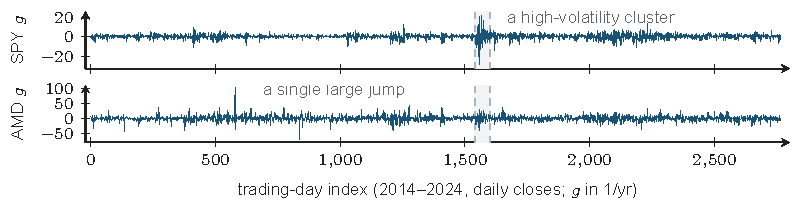
\includegraphics{../figs/Fig-L3a-AMD-Volatility-Clustering.pdf}
  \end{center}

  \vspace{-0.3em}
  \hilite{Volatility clustering}: large-magnitude days arrive in bursts of
  both signs, and the marked weeks are turbulent in both series. One large
  jump is not a cluster.

  \slidenote{Data:}{daily SPY and AMD growth rates, 2014–2024, from the stylized-facts example dataset.}
\end{frame}

\begin{frame}{Diagnosing Volatility Clustering}
  Repeat the ACF calculation using magnitudes.
  For firm $i$, let $\overline{|g|_i}$ be the mean of
  $|g_2^{(i)}|,\ldots,|g_T^{(i)}|$. The magnitude ACF at lag $k$ is given by:
  \[
    \widehat\rho_i(k)=
    \frac{\displaystyle\sum_{t=2}^{T-k}
      \left[|g_t^{(i)}|-\overline{|g|_i}\right]
      \left[|g_{t+k}^{(i)}|-\overline{|g|_i}\right]}
    {\displaystyle\sum_{t=2}^{T}
      \left[|g_t^{(i)}|-\overline{|g|_i}\right]^2}.
  \]

  Positive magnitude autocorrelations across many lags are evidence of
  volatility clustering.

  \slidenote{Main comparison:}{growth-rate autocorrelations can be small while magnitude autocorrelations remain positive.}
\end{frame}

\begin{frame}{Example: Stylized Facts}
  We can now check all three patterns in daily growth-rate data.

  \vspace{0.7em}
  \begin{itemize}\setlength{\itemsep}{0.8em}
    \item Compare observed growth rates with Normal, Laplace, and Student-$t$
      distributions.
    \item Estimate the tail index across several cutoffs.
    \item Compare the ACF of growth rates with the ACF of their magnitudes.
  \end{itemize}

  \slidenote{Example:}{\href{https://github.com/varnerlab/CHEME-5660-CourseRepository-Fall-2026/blob/main/lectures/week-3/L3a/CHEME-5660-L3a-StylizedFacts-Example-Fall-2026.ipynb}{Stylized Facts in Daily Growth Rates}}
\end{frame}

% ==== optional advanced material =============================
\begin{frame}{Optional Advanced Material}
  These examples extend the market-structure discussion.

  \vspace{0.9em}
  \begin{itemize}\setlength{\itemsep}{1em}
    \item \href{https://github.com/varnerlab/CHEME-5660-CourseRepository-Fall-2026/blob/main/lectures/week-3/L3a/advanced/order_book/CHEME-5660-L3a-Advanced-LimitOrderBook-Mechanics-Fall-2026.ipynb}{Limit-Order Book Mechanics}\\
      Match orders, process cancellations, and calculate the prices paid
      by a market order.
    \item \href{https://github.com/varnerlab/CHEME-5660-CourseRepository-Fall-2026/blob/main/lectures/week-3/L3a/advanced/market_impact/CHEME-5660-L3a-Advanced-Market-Impact-Models-Fall-2026.ipynb}{Market Impact Models}\\
      Compare the cost of using the order book with models of how trades
      affect prices.
  \end{itemize}

  \slidenote{Suggested order:}{complete the order-book example first. Neither is required for L3b.}
\end{frame}

% ==== summary ================================================
\begin{frame}{Summary}
  This lecture connected equity trading, price growth, and patterns in market data.

  \vspace{0.8em}
  {\large\textbf{\ink{Key takeaways}}}
  \vspace{0.4em}
  \begin{itemize}\setlength{\itemsep}{0.7em}
    \item \textbf{\ink{Trading determines the price.}}
      Order instructions and available quotes affect where and how a trade fills.
    \item \textbf{\ink{State the units and horizon.}}
      Growth rates, log returns, and their volatilities describe the same
      price changes on different scales.
    \item \textbf{\ink{Check all three patterns.}}
      Growth rates have heavy tails and weak linear autocorrelation;
      their magnitudes remain correlated over time.
  \end{itemize}

  \vspace{0.6em}
  Next, we test a binomial lattice against these patterns.
\end{frame}

% ==== closing ================================================
\transitionframe{That's a wrap. \hilite{What are some of the interesting things
we discussed today?}}

\end{document}
